% Created 2024-01-27 sáb 17:09
% Intended LaTeX compiler: pdflatex
\documentclass[aspectratio=169, usenames,svgnames,dvipsnames]{beamer}
\usepackage[utf8]{inputenc}
\usepackage[T1]{fontenc}
\usepackage{graphicx}
\usepackage{longtable}
\usepackage{wrapfig}
\usepackage{rotating}
\usepackage[normalem]{ulem}
\usepackage{amsmath}
\usepackage{amssymb}
\usepackage{capt-of}
\usepackage{hyperref}
\usepackage{color}
\usepackage{listings}
\usepackage{mathpazo}
\usepackage{gensymb}
\usepackage{amsmath}
\usepackage{diffcoeff}
\usepackage{steinmetz}
\usepackage{mathtools}
\usepackage{fancyvrb}
\DefineVerbatimEnvironment{verbatim}{Verbatim}{fontsize=\tiny, formatcom = {\color{black!70}}}
\bibliographystyle{plain}
\usepackage{siunitx}
\sisetup{per-mode=symbol}
\sisetup{output-decimal-marker={,}}
\DeclareSIUnit{\watthour}{Wh}
\DeclareSIUnit{\wattpeak}{Wp}
\DeclareSIUnit{\watthour}{Wh}
\DeclareSIUnit{\amperehour}{Ah}
\usepackage{steinmetz}
\hypersetup{colorlinks=true, linkcolor=Blue, urlcolor=Blue}
\usepackage[symbol, perpage]{footmisc}
\parskip=5pt
\usetheme{Boadilla}
\usecolortheme{rose}
\usefonttheme{serif}
\author{\href{https://oscarperpinan.github.io}{Oscar Perpiñán Lamigueiro}}
\date{}
\title{Introducción a las Centrales Fotovoltaicas}
\institute[UPM]{Universidad Politécnica de Madrid}
\setbeamercolor{alerted text}{fg=blue!50!black} \setbeamerfont{alerted text}{series=\bfseries}
\AtBeginSubsection[]{\begin{frame}[plain]\tableofcontents[currentsubsection,sectionstyle=show/hide,subsectionstyle=show/shaded/hide]\end{frame}}
\AtBeginSection[]{\begin{frame}[plain]\tableofcontents[currentsection,hideallsubsections]\end{frame}}
\beamertemplatenavigationsymbolsempty
\setbeamertemplate{footline}[frame number]
\setbeamertemplate{itemize items}[triangle]
\setbeamertemplate{enumerate items}[circle]
\setbeamertemplate{section in toc}[circle]
\setbeamertemplate{subsection in toc}[circle]
\hypersetup{
 pdfauthor={\href{https://oscarperpinan.github.io}{Oscar Perpiñán Lamigueiro}},
 pdftitle={Introducción a las Centrales Fotovoltaicas},
 pdfkeywords={},
 pdfsubject={},
 pdfcreator={Emacs 29.1 (Org mode 9.6.11)}, 
 pdflang={Spanish}}
\begin{document}

\maketitle

\begin{frame}[label={sec:orgdae9f28}]{Definición}
Una central fotovoltaica es un sistema fotovoltaico de gran tamaño (del orden de MW) diseñado para la venta de energía a la red eléctrica.

\begin{center}
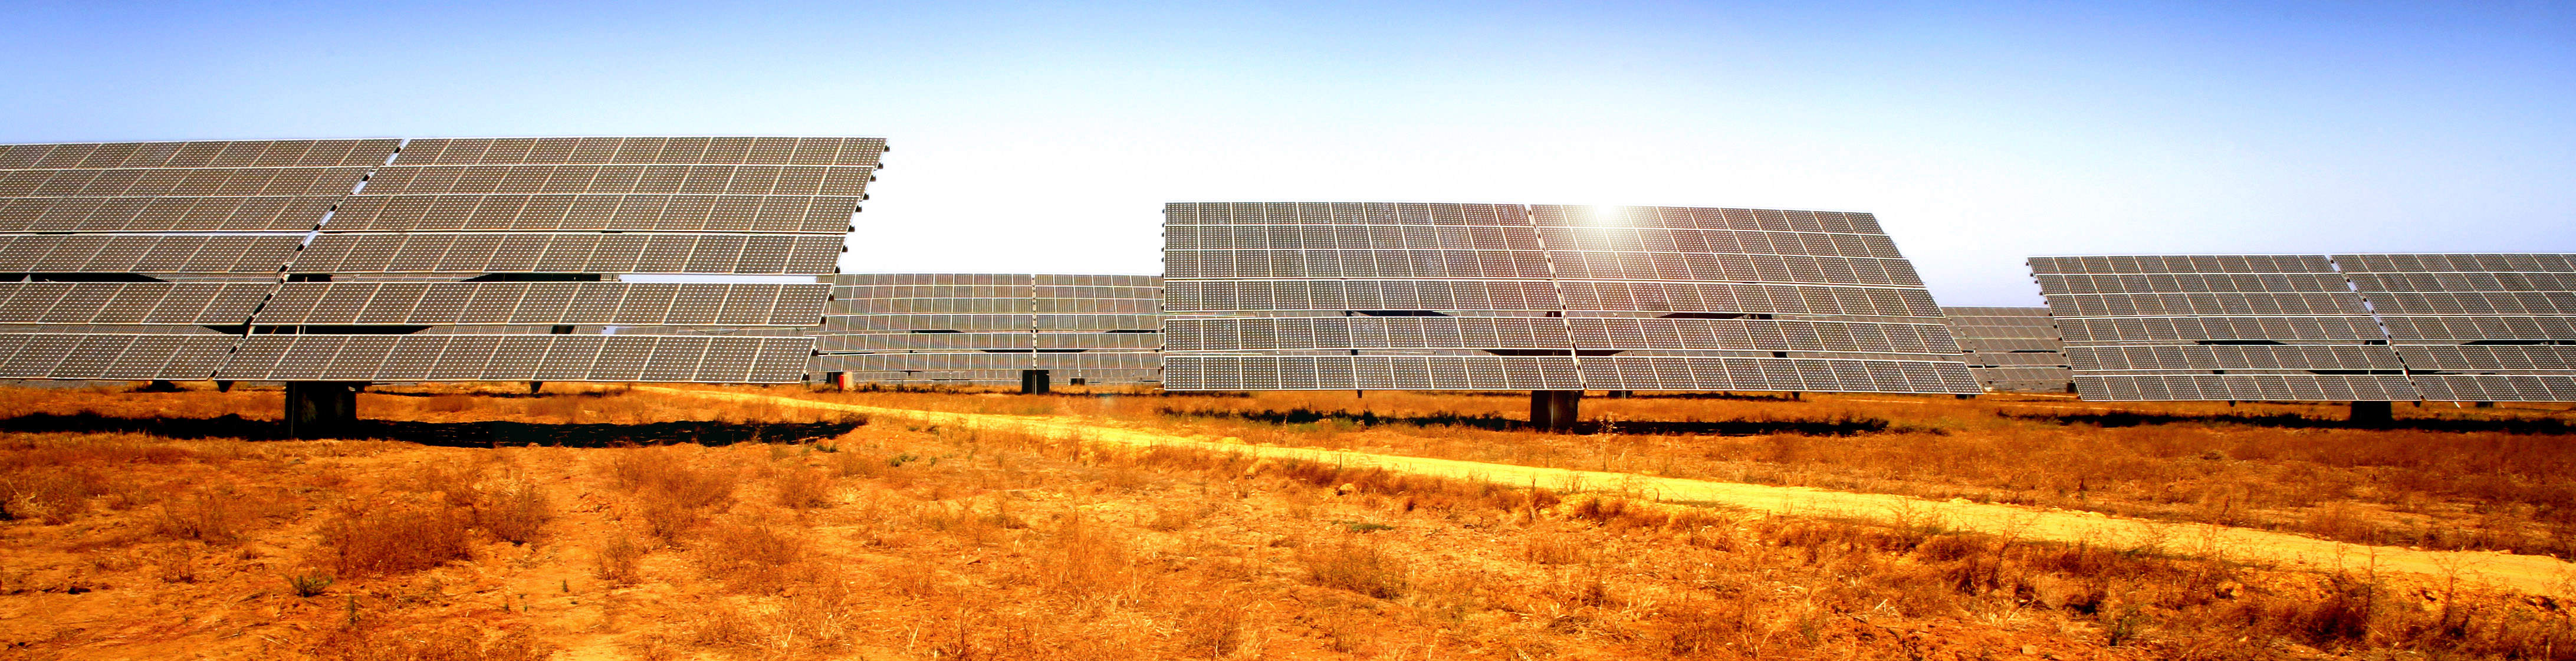
\includegraphics[width=\textwidth]{../figs/carmona_vistaamplia.jpg}
\end{center}
\end{frame}

\begin{frame}[label={sec:org539d0c7}]{Características (1)}
\begin{itemize}
\item Habitualmente se instalan \alert{sobre suelo}, sin estar necesariamente asociadas a un punto de consumo cercano.
\item Como solución a las limitaciones de suelo disponible, están apareciendo \alert{sistemas flotantes} (embalses).
\item Como solución a los conflictos sociales y ambientales por el uso del suelo, están apareciendo \alert{sistemas agrovoltaicos}.
\end{itemize}

\begin{center}
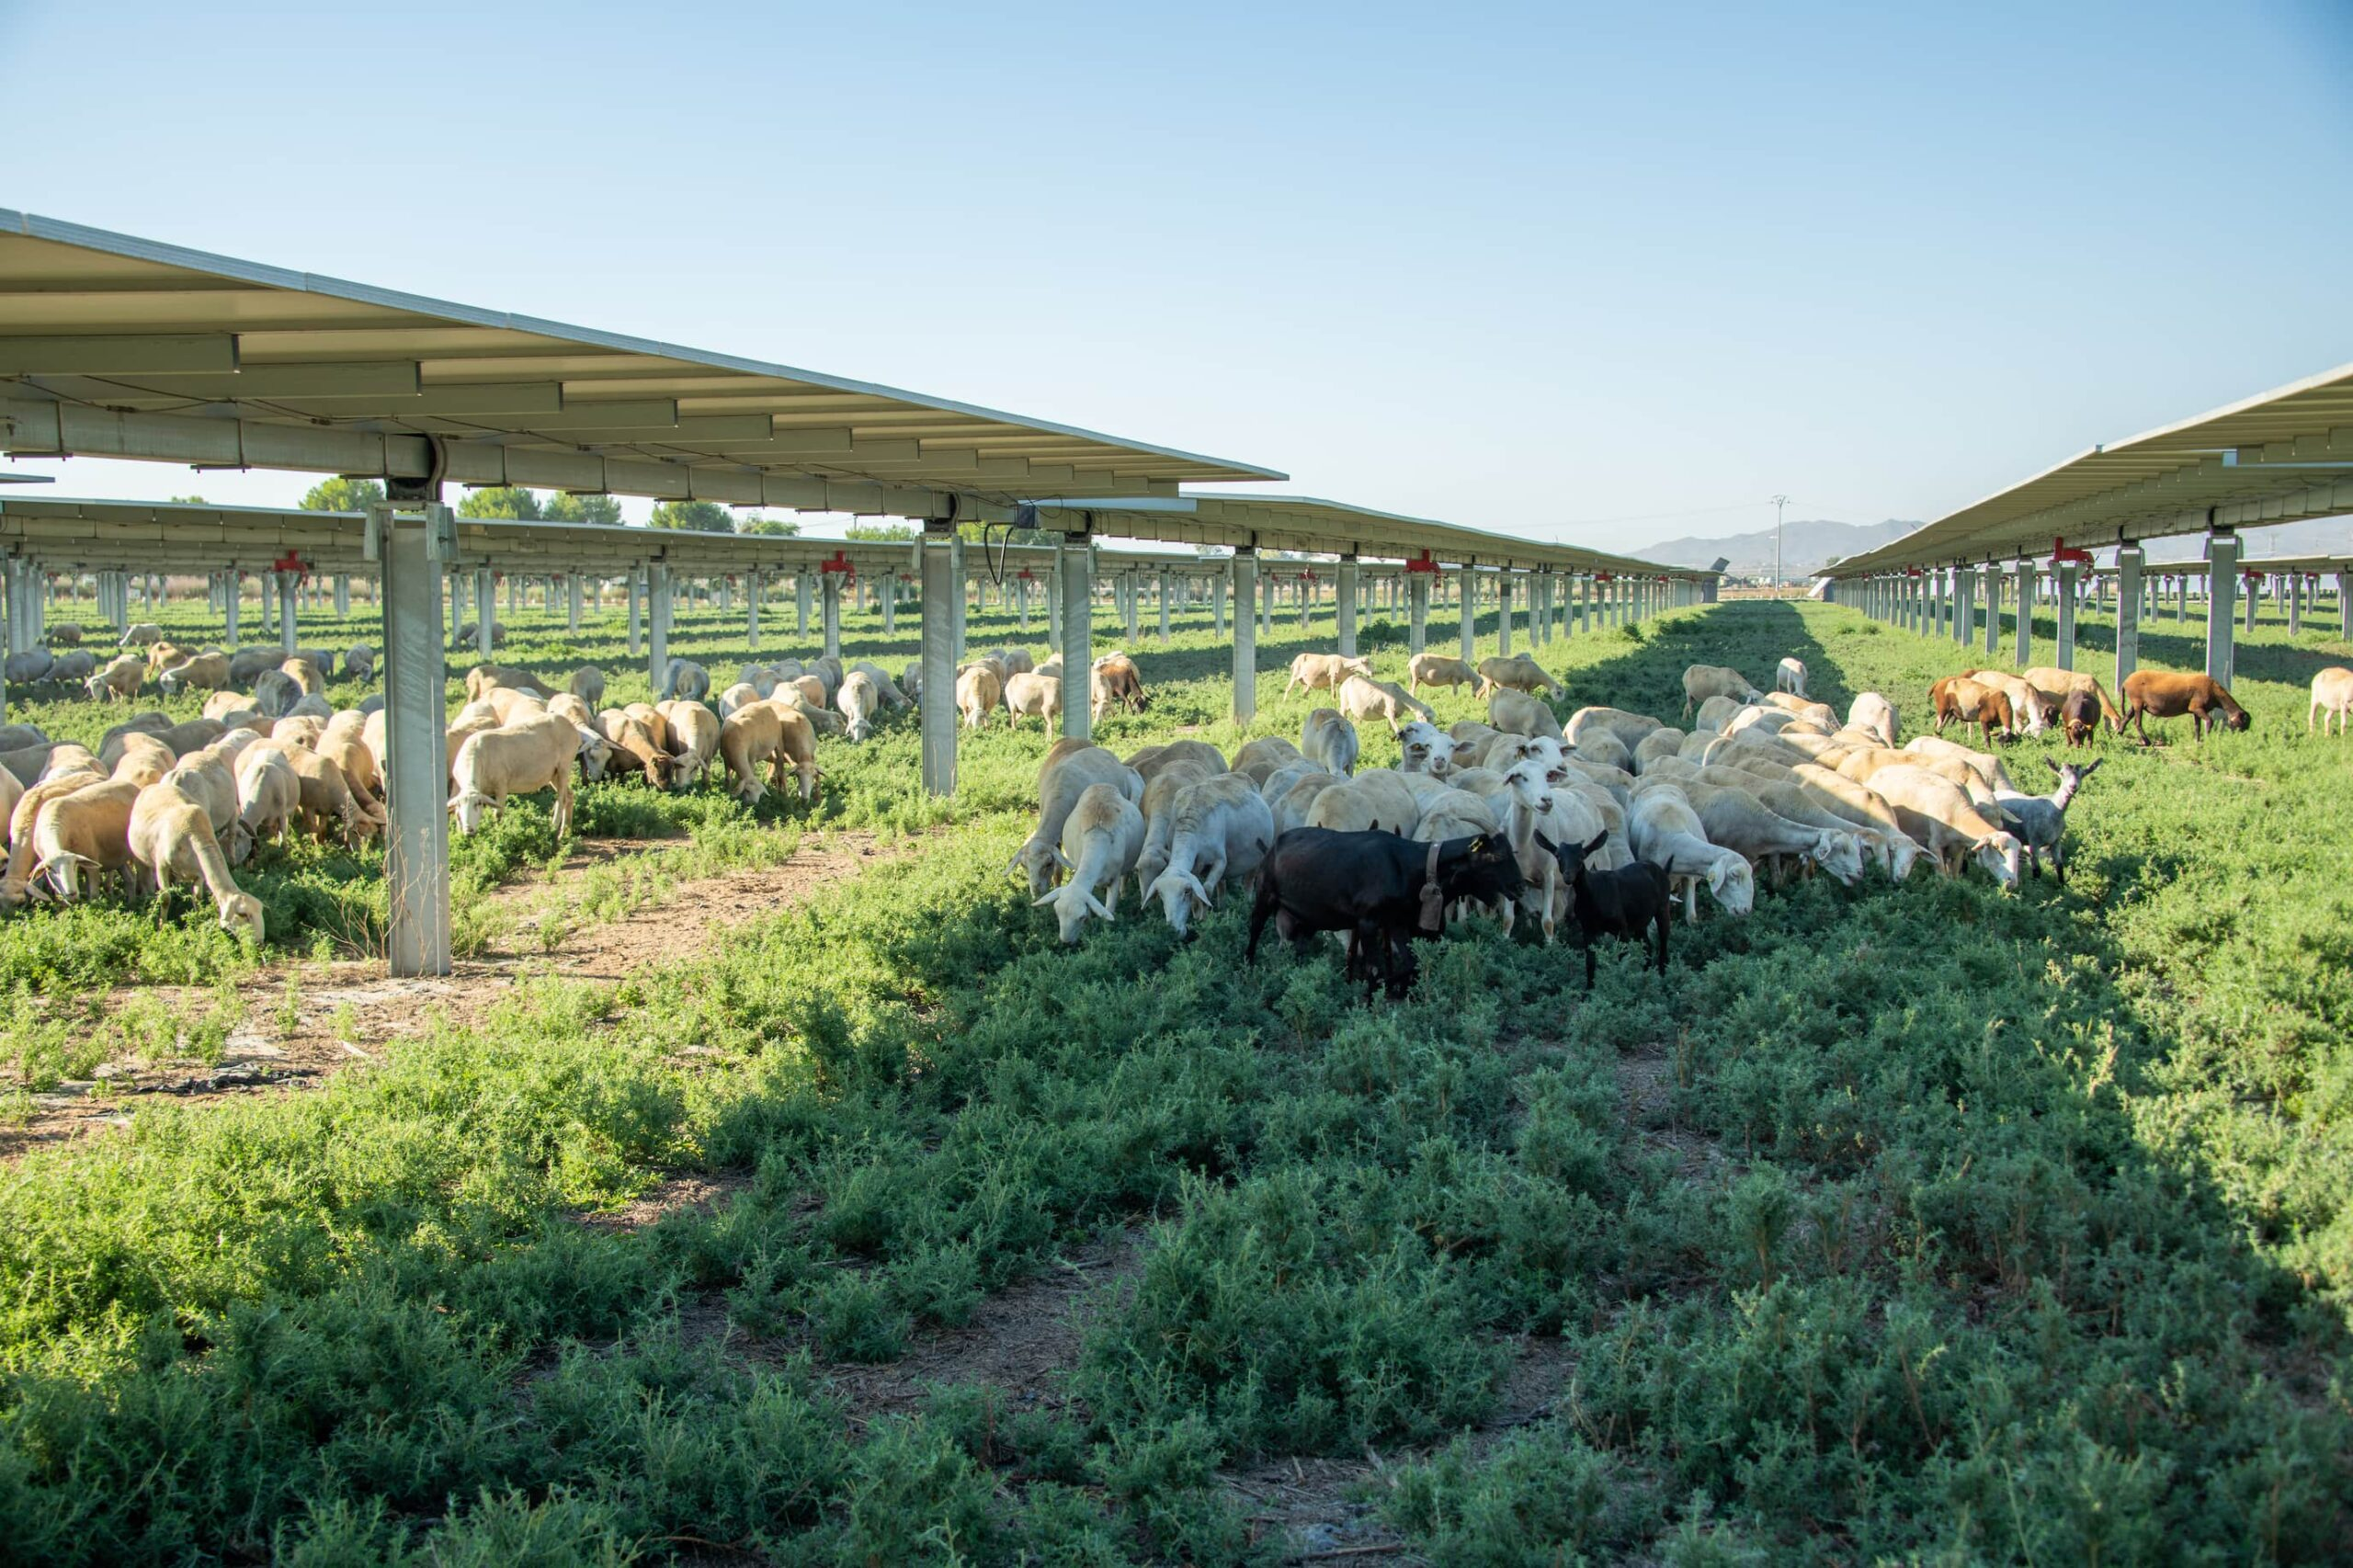
\includegraphics[height=0.5\textheight]{../figs/agrovoltaics.jpg}
\end{center}
\end{frame}


\begin{frame}[label={sec:org9dbd947}]{Características (2)}
\begin{itemize}
\item Se emplean \alert{módulos de gran tamaño} (incluso bifaciales) para reducir los tiempos y costes de instalación.
\item Pueden utilizar \alert{seguidores} para maximizar la producción.
\end{itemize}

\begin{center}
\includegraphics[height=0.5\textheight]{../figs/carmona.jpg}
\end{center}
\end{frame}

\begin{frame}[label={sec:org9f49608}]{Características (y 3)}
\begin{itemize}
\item La inyección de la energía eléctrica se realiza en \alert{Media Tensión}.
\item Incorporan \alert{inversores de gran potencia} y centralizados, y centros de transformación BT/MT.
\item Pueden incorporar \alert{elementos de acumulación electroquímica} para atenuar los efectos de la variabilidad de la irradiancia, y para la prestación de servicios a la red eléctrica.
\end{itemize}

\begin{center}
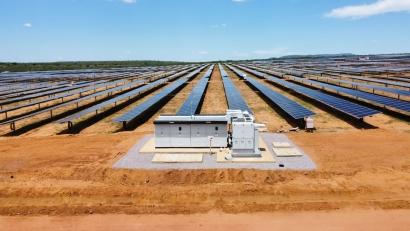
\includegraphics[height=0.5\textheight]{../figs/1power_station_de_ingeteam_en_la_planta_pv_bon_nome.jpg}
\end{center}
\end{frame}

\begin{frame}[label={sec:org5b06b2a}]{Estado del arte (1)}
Las centrales fotovoltaicas superan los 648 GW\footnote{Las cifras corresponden a finales de 2022, y provienen del informe \guillemotleft{}\href{https://iea-pvps.org/trends\_reports/trends-2023/}{Trends in Photovoltaic Applications 2023}\guillemotright{} de la Task 1 de IEA-PVPS.}  de potencia total instalada a nivel mundial (el 55\% de la potencia fotovoltaica total):
\begin{itemize}
\item 254 GW en China,
\item 90 GW en EEUU,
\item 67 GW en India,
\item 34 GW en Japón,
\item 24 GW en España.
\end{itemize}
\end{frame}



\begin{frame}[label={sec:org1d89d1d}]{Estado del arte (2)}
En 2022 se instalaron 120 GW  (frente a 92 GW en 2021 y 84 GW in 2020):
\begin{itemize}
\item 54 GW en China,
\item 14 GW en India,
\item 12,5 GW en EEUU,
\item 5,5 GW en España.
\end{itemize}
\end{frame}
\end{document}
